\chapter{Docker}

\section{关于Docker}

Docker是一个开源的应用容器引擎,让开发者可以打包他们的应用以及依赖包到
一个可移植的容器中,然后发布到任何流行的 Linux 机器上,也可以实现虚拟化。
容器是完全使用沙箱机制,相互之间不会有任何接口。几乎没有性能开销,可以
很容易地在机器和数据中心中运行。最重要的是,他们不依赖于任何语言、框架
包括系统。

\begin{verbatim}
yum install -y docker.io
\end{verbatim}

\section{容器 VS. 虚拟机}

容器为应用程序提供了隔离的运行空间:每个容器内都包含一个独享的完整用户
环境空间,并且一个容器内的变动不会影响其他容器的运行环境,如
图\ref{fig:container}所示。为了能达到这种效果,容器技术使用了一系
列的系统级别的机制诸如利用Linux namespaces来进行空间隔离,通过文件系统
的挂载点来决定容器可以访问哪些文件,通过cgroups来确定每个容器可以利用多
少资源。此外容器之间共享同一个系统内核,这样当同一个库被多个容器使用时,
内存的使用效率会得到提升。

\begin{figure}[!htbp]
  \centering
  \includegraphics{graph/container01.pdf}
    \caption{容器架构模型}
  \label{fig:container}
\end{figure}

对于系统虚拟化技术来说,虚拟层为用户提供了一个完整的虚拟机:包括内核在
内的一个完整的系统镜像。CPU虚拟化技术可以为每个用户提供一个独享且和其他
用户隔离的系统环境,虚拟层可以为每个用户分配虚拟化后的CPU、内存和IO设备
资源,如图\ref{fig:virtualization}所示。

\begin{figure}[!htbp]
  \centering
  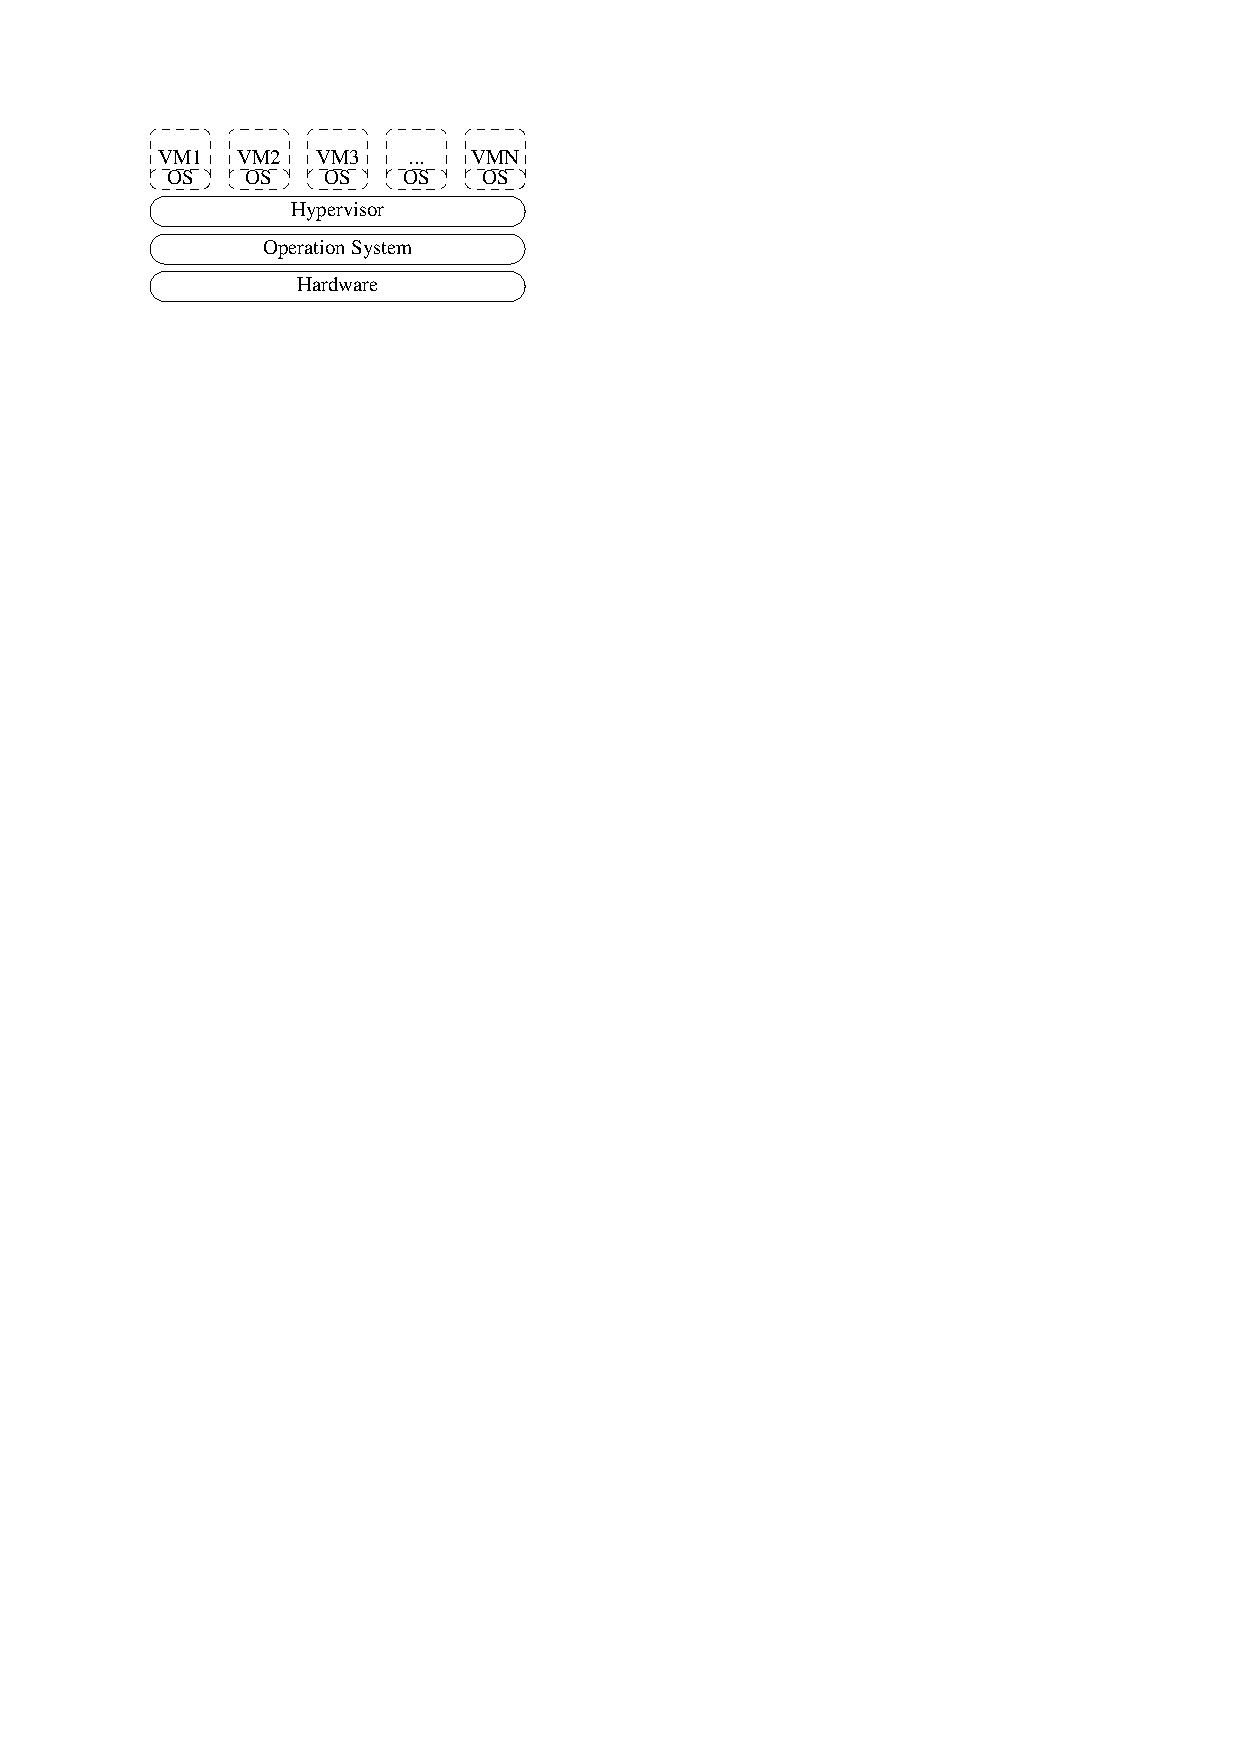
\includegraphics{graph/virtualization01.pdf}
    \caption{虚拟化架构模型}
  \label{fig:virtualization}
\end{figure}

\begin{verbatim}
git config --global user.name "Laven Liu"
git config --global user.email "air.man.six@gmail.com"
\end{verbatim}

\section{Docker简介}
\label{sec:introDocker}

\subsection{Docker与传统虚拟机建构对比}
\label{sec:contrastVM}

\subsection{应用容器虚拟化定位}
\label{sec:dockerDirect}

\subsection{Docker有哪些优势}
\label{sec:dockerAdvance}

\subsection{Docker应用场景}
\label{sec:dockerSec}

\subsection{Docker组成}
\label{sec:dockerComponents}

\section{安装及启动第一台Docker容器}
\label{sec:installDocker}

\section{测试环境}
\label{sec:dockerTestEnv}

Docker章节的演示在Ubuntu14.04 LTS 64位系统上进行演示\footnote{在此之前,
  作者是在CentOS6.5 64位系统上进行演示的,遇到过DeviceMapper的问题,甚
  至有时CentOS还会发生Kernel Panic的现象,故使用了Ubuntu系统进
  行Docker章节的演示。}。演示环境所使用的机器列表如下:

\begin{table}[htbp]
  \centering
    \caption{Docker演示环境机器一览}
    \label{tab:dockerMachines}
    \begin{tabular}{llr}
      \toprule
      主机名     & IP地址 & 说明 \\
      \midrule
      master01.lavenliu.com  & 192.168.20.134 &  主DNS \\
      minion01.lavenliu.com  & 192.168.20.135 &  辅DNS \\
      minion02.lavenliu.com  & 192.168.20.136 &  客户端 \\
      \bottomrule
    \end{tabular}
\end{table}

\subsection{安装Docker}
\label{installDocker}

在安装Docker之前,需要设置Docker官方的镜像源。

\begin{verbatim}
% sudo apt-get update
% sudo apt-get install docker-engine
% sudo status docker
\end{verbatim}

\begin{figure}[hbtp]
  \centering
  \includegraphics{graph/os-arch-mps.pdf}
    \caption{系统架构}
  \label{fig:OSArch}
\end{figure}

\subsection{运行第一台Docker容器}
\label{sec:runFirstDocker}

\section{容器及镜像管理}
\label{sec:containerManagement}

\subsection{容器管理}
\label{sec:containerManage}

\subsection{镜像管理}
\label{sec:dockerImageManage}

\section{构建Docker镜像}
\label{sec:buildDockerImage}

\subsection{手工构建}
\label{sec:buildDockerImgByHand}

\subsection{使用Dockerfile构建}
\label{sec:buildDockerImgByFile}


%%% Local Variables:
%%% mode: latex
%%% TeX-master: t
%%% End:
